    Случайные графы -- один из центральных разделов дискретной математики, расположенный на стыке теории вероятностей, комбинаторики и теории графов.
    Основы теории случайных графов были заложены в 50-х -- 60-х годах прошлого века венгерскими математиками П.~Эрдёшем и А.~Реньи.
    Существует множество моделей случайных графов, разработанных с учётом адекватности их применения в прикладных областях: моделирования социальных, биологических и инфраструктурных сетей. 
    В настоящей работе мы будем иметь дело с \textit{моделью Эрдёша--Реньи}, также называемой \textit{классической моделью} случайного графа.
    % Определение G(N,p)
    
    Многие вопросы этой теории связаны с асимптотическими свойствами случайного графа, то есть с тем, как он ведёт себя при устремлении количества вершин $N$ к бесконечности.
    Удивительным образом оказывается, что для целого класса таких вопросов можно, совершенно не вдаваясь в сущность конкретного вопроса, дать на него едва ли не исчерпывающий ответ.
    Точнее говоря, если про случайный граф спрашивается ``Как при увеличении числа вершин до бесконечности будет вести себя вероятность того, что граф обладает свойством $A$?'', то во многих случаях можно заранее сказать: ``Будет стремиться к 0 или к 1''.
    В этом состоит суть теорем, называемых \textit{законами нуля или единицы}, уточнению условий применимости которых посвящена данная работа.
    
    Чтобы перейти к изложению известных результатов о законах нуля или единицы, дадим определения основным понятиям и сформулируем теоремы, касающиеся важных для нас свойств случайного графа $G(N,p)$ (см. \cite{survey2015}).
    
    Пусть $N \in \N$, $0 \leq p \leq 1$. Рассмотрим множество $\Omega_N = \{G = (V_N , E)\}$, $|\Omega_N| = 2^{C_N^2}$ всех неориентированных графов без петель и кратных ребер с множеством вершин $V_N = \{1, \ldots, N \}$.
    
    %NOTE: Максим: Случайные графы бывают независимы, чего нельзя сказать про элементарные исходы
    % \Def \textit{Случайный граф $G(N, p) \in \Omega_N$  в модели Эрдёша-Реньи} -- это элементарный исход в вероятностном пространстве $(\Omega_N, \P_{N.p}, 2^{\Omega_N})$, где  распределение $\P_{N.p}$ определяется формулой $\P_{N.p}(G) = p^{|E|}(1-p)^{C_N^2-|E|}$
    
  \Def \textit{Случайный граф $G(N, p)$  в модели Эрдёша-Реньи}~--- это случайный элемент со значениями во множестве $\Omega_N$ и распределением $\P_{N.p}(G) = p^{|E|}(1-p)^{C_N^2-|E|}$, определённом на $\mathscr{F}=2^{\Omega_N}$.
  
  Иначе говоря, это полный граф на $N$ вершинах, в котором каждое ребро независимо от других рёбер удаляется с вероятностью $1-p$.
  Параметр $p$ называют вероятностью проведения ребра.
    
    \Def Для произвольного языка $\F$, случайный граф $G(N, p)$ \textit{подчиняется закону нуля или единицы для языка $\F$},
    если для любой формулы $\varphi$ из языка 
    $\F$  выполнено
    $\lim_{N \rightarrow \infty} \P(G(N, p) \vDash \varphi) \in \{0, 1\}$.
    
    Введём обозначение $\LL$ для языка первого порядка с сигнатурой, в которую входят только двуместные предикаты равенства ($=$) и смежности ($\sim$).
    За точными определениями можно обратиться, например, к
    \cite{shen}, а здесь мы ограничимся лишь напоминанием о том, что формулы языка первого порядка~--- это предложения, составленные из символов, обозначающих переменные: 
    $x,y,z,x_1,\ldots$, 
    логических связок 
    $\wedge, ~\neg, ~\vee$, 
    кванторов 
    $\exists, ~\forall$ и 
    предикатных символов (в нашем случае
    $\sim, ~ =$).
    Например, формула, утверждающая, что диаметр графа (расстояние между двумя наиболее удалёнными друг от друга вершинами, измеряемое в рёбрах) не превосходит 2, выглядит так:
    \[
    \forall x \forall y ~ x=y \vee x\sim y \vee \left( \exists z ~ x \sim z \wedge z \sim y \right).
    \]
    
    Всюду далее $E(G)$ будет обозначать множество вершин графа $G$, а $V(G)$~--- множество его рёбер.
    
    \Def \textit{Плотность} графа $G$ 
   \[ \rho(G) = \frac {|E(G)|}{|V(G)|} .\]
   
   \Def \textit{Максимальная плотность} графа $G$
     \[ \rho^{max}(G) = \max_{H \subseteq G} \frac {|E(H)|}{|V(H)|} .\]
    
    \Def Граф $G$ называется \textit{сбалансированным}, если 
    \[ \rho^{max}(G) = \rho(G) .\]
    
    \Def Граф $G$ называется \textit{строго сбалансированным}, если 
    \[\rho^{max}(G) = \rho(G) > \max_{H \subsetneq G} \frac {|E(H)|}{|V(H)|} .\]
    
    \Def Функция $f(N): \N \rightarrow [0,1]$ называется \textit{пороговой функцией} для свойства $\varphi$ и случайного графа $G(N,p)$, если при $p(N) \ll f(N)$ вероятность $\P(G(N,p) \vDash \varphi)$ стремится к нулю (единице), и, наоборот, при $p(N) \gg f(N)$ вероятность $\P(G(N,p) \vDash \varphi)$ стремится к единице (нулю).
    
    Здесь и далее $f(N) \ll g(N)$ означает $f(N) = o(g(N))$.
     
В 1960 г. П. Эрдёш и А. Реньи
доказали теорему об условиях справедливости утверждения ``$G(N, p)$ содержит копию данного сбалансированного графа'' \cite{erdHos1976evolution}. 
Позже этот результат получил следующее обобщение.\\
\begin{theorem} (А. Ручински, А. Винс, 1985, \cite{rucinski1985balanced}) 
\label{th:ruchinski}
Пусть дан некоторый граф $H$.
Функция $N^{-1/\rho^{max}(H)}$ является пороговой для случайного графа $G(N,p)$ и свойства содержать копию графа $H$ в качестве подграфа.
\end{theorem}


Для нас очень важно то, что при $p = N^{-1/\rho^{max}(H)}$ вероятность содержать подграф $H$ не стремится ни к нулю, ни к единице.
Это утверждение, содержащееся в следующей теореме, даёт удобный способ доказывать отсутствие законов нуля или единицы для $G(N, N^{-\alpha}), ~\alpha \in \Q$.

\begin{theorem} (Б. Боллобаш, 1981, \cite{bollobas1981threshold}). 
\label{th:bollobash}
Пусть $H$~--- строго сбалансированный граф, $a$~--- количество автоморфизмов графа $H$, $p = N^{-1/ \rho^{max}(H)}$.
Тогда
\[N_H \xrightarrow[N\rightarrow \infty]{d} Poiss(1/a). \]
Здесь $N_H$~--- количество копий графа $H$ в $G(N, p)$, $Poiss(1/a)$~--- пуассоновская случайная величина со средним $1/a$.
\end{theorem}
Из последней теоремы и доказанного в \cite{rucinski1986strongly} утверждения о том, что для любого $\alpha \in (0,1] \cap \Q$ существует строго сбалансированный граф $H$ с плотностью $\rho(H) = 1/\alpha$, следует, что $G(N,N^{-\alpha})$ не подчиняется закону нуля или единицы для языка $\LL$ при всех рациональных $\alpha$ из интервала $(0,1]$.
Это верно и для $\alpha = (k+1)/k,~ k > 0$, т.к. для каждого из таких $\alpha$ существует дерево с соответствующей плотностью.
При $\alpha > 2$ граф $G(N, N^{-\alpha})$ асимптотически почти наверное пуст, и, следовательно, подчиняется закону нуля или единицы.
Оказывается, что при всех прочих $\alpha$ случайный граф $G(N, N^{-\alpha})$ также подчиняется закону нуля или единицы.
Итак, имеет место следующая теорема.
\begin{theorem} (Дж. Спенсер, С. Шелах, 1988, \cite{shelah1988zero})
\label{th:spencer}
Случайный граф $G(N, N^{-\alpha})$ подчиняется закону нуля или единицы для языка $\LL$ при всех $\alpha$, кроме $\alpha \in \left((0,1] \cap \Q \right) \cup \{(k+1)/k ~|~ k \in \N \}$.
\end{theorem}

О том, сохраняется ли закон нуля или единицы, когда вероятность проведения ребра лежит в ``промежутках'' между степенными функциями, говорят следующие теоремы.

\begin{theorem} (Дж. Спенсер, С. Шелах, 1988 \cite{shelah1988zero}, \cite{compton1989laws})
\label{th:spencer intermediate}
$G(N, p)$ подчиняется закону нуля или единицы для языка $\LL$ в следующих случаях:
\begin{enumerate}
    \item $N^{-1 - \frac{1}{k}} \ll p(N) \ll N^{-1-\frac{1}{k+1}},~ k \in \N. $
    \item $N^{-1 -\eps} \ll p(N) \ll N^{-1}~ \forall \eps > 0.$
    \item $N^{-1} \ll p(N) \ll N^{-\frac{\ln{N}}{N}}.$
    \item $N^{-\frac{\ln{N}}{N}} \ll p(N) \ll N^{-1 + \eps}~ \forall \eps > 0.$
    \item $N^{-\eps} \ll p(N)~ \forall \eps > 0.$
\end{enumerate}
\end{theorem}


\begin{theorem} \cite{spencer2013strange}
Для любого иррационального $\alpha \in (0,1)$ случайный граф $G(N,N^{-\alpha +o(1)})$ подчиняется закону нуля или единицы для языка $\LL$.
\end{theorem}

Чтобы прояснить содержание теоремы $\ref{th:spencer intermediate}$, расскажем подробнее о том, как меняются  асимптотические свойства графа Эрдёша--Реньи при изменении асимптотики вероятности проведения ребра.
Легко видеть, что при $p(N) = o(N^{-2})$ в случайном графе $G(N,p)$ асимптотически почти наверное нет рёбер: из неравенства Маркова, вероятность найти в нём хотя бы одно ребро $\P(|E| \geq 1) \leq \E |E| = \frac{1}{2} N(N-1)p(N) \rightarrow 0$.
При переходе через $\alpha = 2$ в графе появляются изолированные рёбра, а при $p(N) = N^{-1 - \frac{1}{k}}$, как следует из теорем \ref{th:ruchinski}, \ref{th:bollobash} в случайном графе появляются деревья на $k$ вершинах.
В процессе перехода через $\alpha = 1$ в случайном графе выделяется так называемая ``гигантская компонента'': если $p(N)=c/N,~ c < 1$, то асимптотически почти наверное \textit{(а.п.н)} каждая компонента связности случайного графа содержит не более $\beta (c) \ln{N} $ вершин;
если $p(N)=c/N,~ c > 1$, то в случайном графе а.п.н. имеется компонента связности с числом вершин, превосходящим $\gamma(c)N$, то есть растущим линейно с ростом $N$\cite{erdos1959random} \cite{erdos1960evolution} \cite{raigor2010models}.
Следующая интересная точка на пути увеличения вероятности проведения ребра (в смысле асимптотики)~--- это $\ln{N}/N$, пороговая функция для свойства связности.
Если $p(N) = c \frac{\ln{N}}{N}$, то при $c < 1$ случайный граф а.п.н. не связен, а при $c > 1$ он а.п.н является связным\cite{raigor2010models}.
\begin{figure}
  \centering
  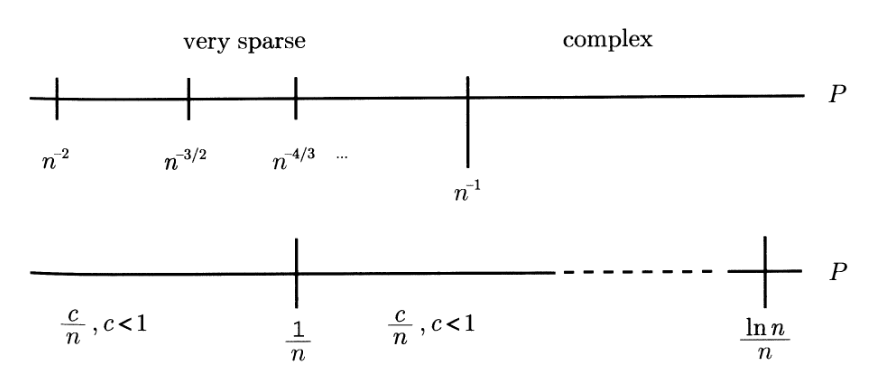
\includegraphics[scale=0.5]{picrel/density.png}
  \caption{Условное соответствие между асимптотикой $p(N)$ и ``разреженностью'' случайного графа. Пороговые функции для свойств ``содержать дерево на $k$ вершинах'', ``содержать гигантскую компоненту'', ``быть связным''}
  \label{fig:density}
\end{figure}

Ниже мы сформулируем для других языков несколько теорем, аналогичных теореме \ref{th:spencer}.

\Def Язык $\LL^k$~--- подмножество $\LL$, содержащее предложения, в которые входят не более $k$ переменных.

На языке $\LL^3$ для любого натурального $d$ можно выразить, например, свойство ``иметь диаметр не более $d$'': 
\[
\psi_d = \forall x \forall y ~ x = y \vee x \sim y \vee \left( \exists z ~ x\sim z \wedge z \sim y \right)
\vee  \left( \exists z ~ x\sim z \wedge \left( \exists x ~ z \sim x \wedge x \sim y \right) \right) \vee \ldots
\]

\Def Язык $\LL^k_{\infty, \omega}$ включает в себя предложения конечной или счётной длины, в которые входят не более $k$ переменных.

На языке $\LL^3_{\infty, \omega}$ можно выразить, например, свойство ``быть связным'': $\psi = \bigvee_{d=1}^\infty \psi_d$.
Это свойство невыразимо в $\LL$.

\Def \[\LL^\omega_{\infty, \omega} = \bigcup_k \LL^k_{\infty, \omega} \]

\begin{theorem}
Случайный граф $G(N, N^{-\alpha})$ подчиняется закону нуля или единицы для языка $\LL^\omega_{\infty, \omega}$ при $\alpha \in (1,2] \setminus \{(k+1)/k ~|~ k \in \N \}$ (Дж. Линч, 1993  \cite{lynch1993infinitary}) и $\alpha > 2$.
Закон нуля или единицы не выполнен при $\alpha \in (0,1]$ (С. Шелах, 2017 \cite{shelah2017failure})  и $\alpha \in \{(k+1)/k ~|~ k \in \N \}$.
\end{theorem}

\begin{theorem} (М. MакАртур, 1997 \cite{mcarthur1997asymptotic})
Для любого $\alpha < \dfrac{1}{k-1}$ случайный граф $G(N, N^{-\alpha})$ подчиняется закону нуля или единицы для языка $\LL^k_{\infty, \omega}$.
\end{theorem}

Ниже дано неформальное определение кванторной глубины формулы.
Формальное определение есть, например, в \cite{shen}.

\Def \textit{Кванторная глубина} формулы~--- наибольшее число вложенных кванторов в формуле.

\Def Язык $\LL_k$~--- подмножество $\LL$, включающее формулы с кванторной глубиной не более $k$.

\begin{theorem}(М. Е. Жуковский, 2012, \cite{zhukovskii2012zero}). Пусть $p=N^{-\alpha}$, $0 < \alpha < 1/(k - 2)$. 
Тогда случайный граф $G(N, p)$ подчиняется закону нуля или единицы для языка $\LL_k$.
\end{theorem}